\section{Sweep Mapping}
\index{sweep mapping}\index{Mapping!SweepMapping}\index{Mapping!make a 3D mapping by extruding a 2D mapping}

The SweepMapping can be used to create these types of mapping's,
\begin{description}
  \item[sweep]: sweep a curve or surface in the $x-y$ plane along a 3D curve.
  \item[extrude]: extrude a curve or surface in the $z$ direction.
  \item[tabulated-cylinder] : generate a surface from a 3D curve by extruding along a specified line.
\end{description}

\subsection{Sweep}

The {\bf sweep} option of the 
SweepMapping will take a planar reference surface $\Sv(r_1,r_2)$ (or reference curve $ \Sv(r_1)$)
and form a three-dimensional volume (or surface) by sweeping the reference surface along a 
3D `sweep-curve' $\Cv(r_3)$. 

The formula defining the sweep mapping is
\begin{displaymath}
\Xv(r_1,r_2,r_3)=\Big\{ \Mv(\rv)~\left[{\Sv}(r_1,r_2) - \cv_0\right]\Big\}~\alpha(r_3)+{\Cv}(r_3)
\end{displaymath}
where 
\begin{align*}
 \Sv & \quad\mbox{: the reference surface (or reference curve) to be swept.}\\
 \Cv & \quad\mbox{: the curve used for sweeping, the {\it sweep-curve}.}\\
 \Mv & \quad\mbox{: a rotation-translation matrix defined from $\Cv$ and $\Sv$.} \\
 \alpha(r_3) & \quad\mbox{: a scaling function.} \\
 \cv_0 & \quad\mbox{a vector used to centre the sweep mapping in different ways.} 
\end{align*}


% Since the centre of the reference surface may not correspond to the starting point 
% of the sweep curve it is necessary to 
The vector $\cv_0$ determines the centering of the SweepMapping with respect to the
reference surface.
There are three options for specifying the centering of the SweepMapping,
\begin{alignat*}{3}
 \cv_0 & = 0  && \quad\mbox{: the centering is based on the sweep curve}\\
 \cv_0 & = \overline{\Sv}(\cdot,\cdot)&&   \quad\mbox{: the centering is based on the reference surface.}\\
 \cv_0 & = \mbox{user-specified} && \quad\mbox{: the centering is user specified.}
\end{alignat*}
Here $\overline{\Sv}(\cdot,\cdot)$ is the centroid of the reference surface. 


The initial rotation-translation matrix $\Mv(r_1,r_2,0)$ will be chosen to translate the reference surface
so that it's centroid, $\overline{\Sv}(\cdot,\cdot)$,  is located at the point $\cv_0$.
The centroid is defined as the average value of the grid point locations,
 \[
	\overline{\Sv}(\cdot,\cdot) = {\sum_{i_1=0}^{n_1}\sum_{i_2=0}^{n_2} \Sv_{i_1,i_2} \over (n_1+1)~(n_2+1) } ~.
\]
$\Mv(r_1,r_2,0)$ will also 
rotate the reference surface to align with the tangent to the sweep-curve. After this rotation the
the normal to the rotated reference surface will be parallel to the initial tangent 
of the the sweep-curve, $\Cv'(0)$ . The {\bf orientation} parameter ($+1$ or $-1$) will determine whether
the normal to $\Sv$ is in the same or opposite direction to the tangent to the sweep curve.
Thus if the sweep mapping appears `inside-out' one should change the orientation. Instead of changing the
orientation one could also reverse the parameterization of the sweep curve.


{\bf This needs to be finished}

\vskip2\baselineskip
{\bf Here is the old documentation.}


\underline{\underline{Purpose}}:\\
Given a planar surface (or curve) $\Sv(r_1,r_2)$ (or $ \Sv(r_1)$), and a 
$3D$ curve $\Cv(r_3)$, we would like to 
generate a $3D$ volume or surface by sweepping $\Sv$ perpendicularly
to $\Cv$ in such a way that the center of each $\Sv_k$ ring lie on
the curve $\Cv$. At $r_3 = 0$, it is assumed that $\Sv = S_0$ is
orthogonal to $\Cv$ and the tangent to $\Cv$ coincide with the
normal $\nv $ to $\Sv$. To make sure that the center of $\Sv =
S_0$ lies at $\Cv(0)$, We first find the center $(x_0,y_0,z_0)$ as the
average of all the points that make up the sweep surface $\Sv$, namely
\[
\xv_0={\sum_{i=0}^n {\xv_i}\over n+1}, 
\]
Then a translation that maps $\Cv(0)$ to $(x_0,y_0,z_0)$ is applied 
to $\Cv$.
\\
\\
\underline{\underline{Strategy}}:\\
With a sufficient number of grid points in each direction, 
we incrementally compute the matrix transformation to be used the
following way. At $k=0$ corresponding to $r_3=0$, the identity matrix is
used since $\Sv$ and $\Cv$ satisfy the required conditions and $\Sv_0 = \Sv$. 
For $k>0$, the ring $\Sv_k$ is gotten from the ring $\Sv_{k-1}$
the following way:\\
A translation that maps the center of $\Sv_{k-1}$ (which is the same
point as $\Cv_{k-1}$) to the point $\Cv_k$ is applied to $\Sv_{k-1}$. A
rotation is then applied to the resulting points is such a way that the
unit normal to the surface $\Sv_{k-1}$ coincides with the tangent to the
curve $\Cv$ at the point $C_k$. To implement this,
the unit vector $\nv_0$  of the surface $\Sv_{k-1}$ is chosen to 
be the first vector in a new orthonormal basis. The second basis vector 
$\nv_1$ is given by $\nv_1 = {n_0\times t \over \| n_0\times t\|}$
where $\tv = {\partial C (r_3+\Delta r_3) \over \partial r_3}$. The third 
basis vector $\nv_2$ is given by $\nv_0\times n_1\over \|n_0\times n_1\|$. In the
new coordinate system, the rotation is about $\nv_1$ with center at
$C_k$. Since $n_0$ is rotated to coincide with $t$, the rotation angle
is given by $\cos \theta = n_0 \cdot t$ and $\sin \theta = t \cdot n_2$.
The overall matrix transformation is therefore a product of three matrices; 
first the matrix transformation from the canonic basis of the
3D vector space to the basis $(n_0, n_1, n_2)$, the rotation of angle
$\theta$ with center
$(0,0,0)$ around $\nv_1$ and finally the matrix transformation from the
basis $(n_0, n_1, n_2)$ to the canonic basis.\\
For the simplification of the mapping calculations, the discrete values 
of the global transformation $M(r_{1k},r_{2k},r_{3k})$ are considered 
as the points for three splines. With these splines we can calculate the 
image of any triplet 
$(r_1,r_2,r_3)$. If $\alpha (r_3)$ is the value of the scalar we will multiply
(also stored in a spline), the image $\Xv(r_1,r_2,r_3)$ is given by\\
\begin{displaymath}
\Xv(r_1,r_2,r_3)=\left\{M(r_1,r_2,r_3)*\left[{\Sv}(r_1,r_2) - {\Cv}(0)\right]\right\}\alpha(r_3)+{\Cv}(r_3)
\end{displaymath}
\\
\\
\underline{\underline{Remark}}\\
At the limit ($\Delta r_3 \rightarrow 0$) corresponding to  the continuous case, the basis $(n_0, n_1, n_2)$ becomes proportional to ${\partial C(r_3)
\over \partial r_3},\, {\partial^2 C(r_3) \over \partial r_3^2}, \,
{\partial C(r_3) \over \partial r_3} \times {\partial^2 C(r_3) \over
\partial r_3^2}$. In fact when $\Delta r_3$ is very small then
\begin{eqnarray*}
n_1 & \approx & {\partial C(r_3) \over \partial r_3} \times {\partial C(r_3 + \Delta r_3) \over \partial r_3}\\
n_1   & \approx & {\partial C(r_3) \over \partial r_3} \times \left(
{\partial C(r_3) \over \partial r_3} + \Delta r_3 {\partial^2 C(r_3)
\over \partial r_3^2} + \cdots \right)\\
    & \approx &  \Delta r_3 {\partial C(r_3) \over \partial r_3}\times
    {\partial^2 C(r_3) \over \partial r_3^2}
\end{eqnarray*}
\vskip\baselineskip
\noindent{Acknowledgement:} Thanks to Thomas Rutaganira for creating the first version of the SweepMapping.

%% Here are the description of some functions of the class
%% \input SweepMappingInclude

\subsection{Examples}


The command file {\bf Overture/sampleMappings/aorticArch.cmd} generates the mappings
for a model of the aortic arch shown in figure \ref{fig:aorticArch}.
\begin{figure}
% \centerline{\epsfxsize=\textwidth \epsffile{fourpipes.eps}}
\begin{center}
  \includegraphics[width=9cm]{\figures/aorticArch}
  % \epsfig{file=aorticArch.ps,width=.6\linewidth}
\end{center}
\caption{The SweepMapping is used to generate mappings for the aortic arch.}\label{fig:aorticArch}
\end{figure}

Figure~\ref{fig:stadium} shows the grids generated by the SweepMapping for a model of a stadium.
\begin{figure}
\begin{center}
  \includegraphics[width=9cm]{\figures/stadium2d}
  \includegraphics[width=9cm]{\figures/stadium3d}
  % \epsfig{file=stadium2d.ps,width=.45\linewidth}
  % \epsfig{file=stadium3d.ps,width=.45\linewidth}
\end{center}
\caption{The SweepMapping is used to generate mappings for a stadium.}\label{fig:stadium}
\end{figure}


% The following command file generates the geometry for the aortic arch.
% \begin{multicols}{3}
% {\ttfamily \scriptsize
% % \labelstyle{\ttfamily}
% % \keywordstyle{\ttfamily}
% % \commentstyle{\ttfamily}
% % \stringstyle{\ttfamily}
% % \postlisting{\bigbreak}
% \listinginput[1]{1}{fourpipes3.cmd}
% }
% \end{multicols}
% This lead to the mapping shown in figure \ref{fig:aorticArch}.
% \begin{figure}
% % \centerline{\epsfxsize=\textwidth \epsffile{fourpipes.eps}}
% \begin{center}
% \epsfig{file=fourpipes3.ps,width=.75\linewidth}
% \end{center}
% \caption{The SweepMapping is used to generate mappings for the aortic arch.}\label{fig:aorticArch}
% \end{figure}
